\section{Implementation}
As this was part of our access management platform and requirement for our project, we implemented this floorplan also in our web application.

\begin{figure}[!hb]
	\centering
	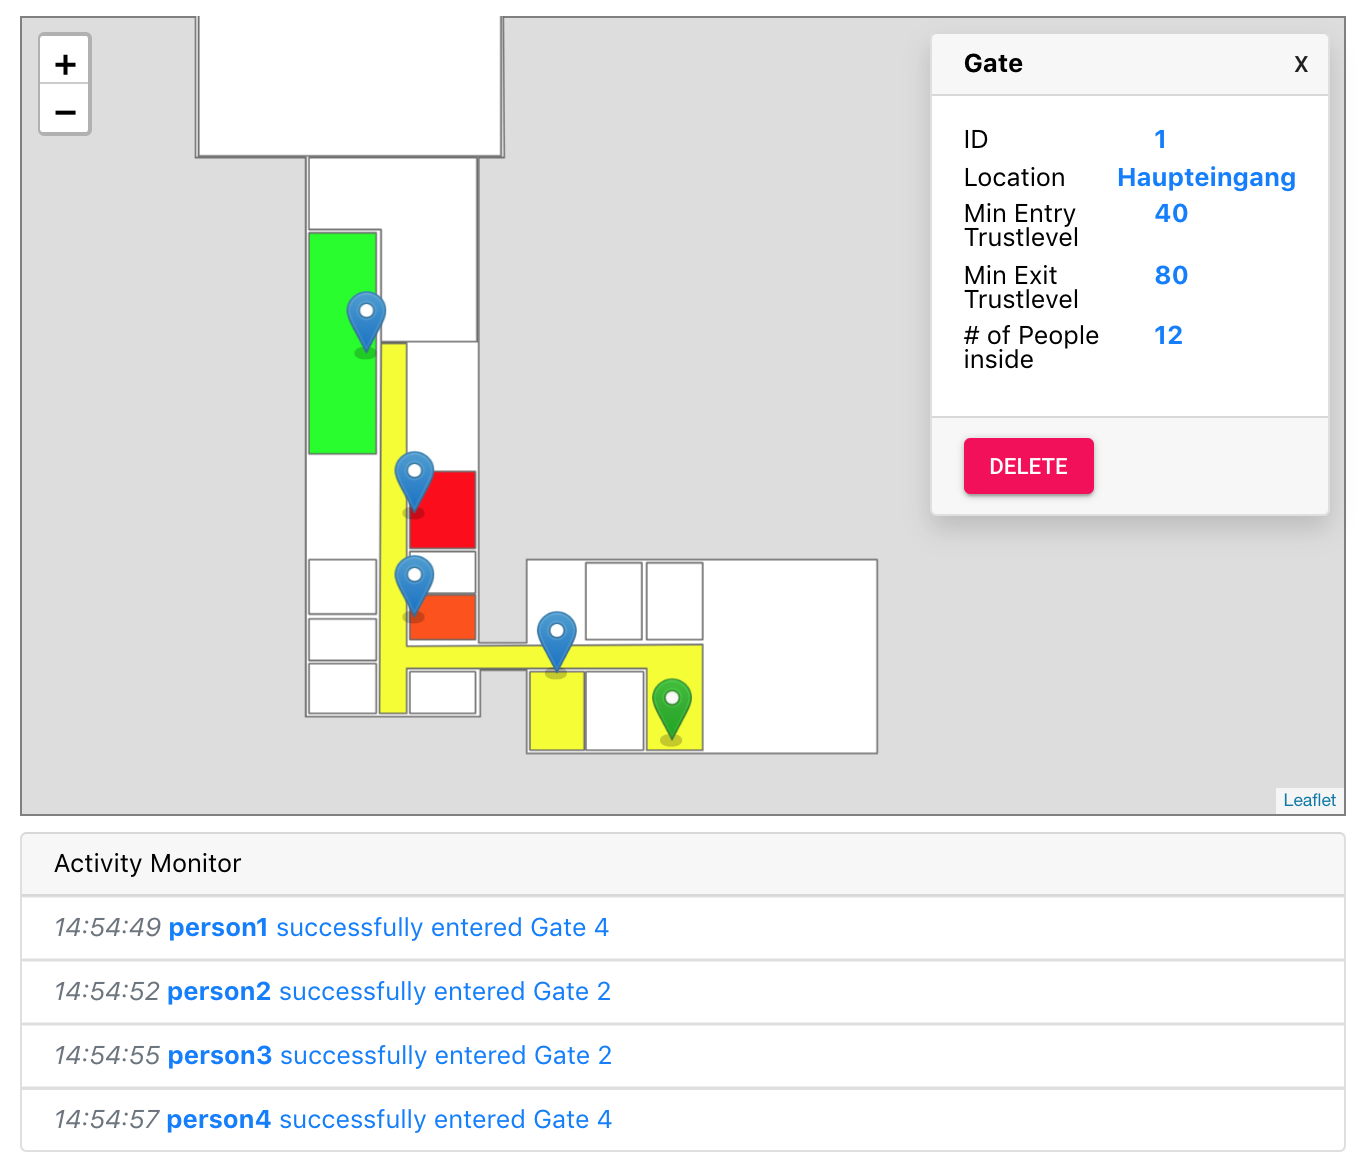
\includegraphics[width=0.9\linewidth]{images/FloorplanScreenshot}
	\caption{Screenshot of the implemented interactive floorplan}
	\label{fig:FloorplanScreenshot}
\end{figure}

\subsection{Display of Indoor features}
\label{Display of Indoor features}

Reinladen von GeoJSON

Code zeigen?

Hier erwaehnen das jedes feature eine ID benoetigt und so.

\subsection{Adding of markers}
\label{Adding of markers}

When adding a marker its linked with the underlying room id.

\begin{lstlisting}[label=addMarkers]
handleClickOnRoom = (event) => {
        this.addMarker(event.latlng, { gateId: undefined, assignedRoomId: event.target.feature.id }, true);
    };

    addMarker(latlng, info = { gateId: undefined }, setAsSelected = false) {
        const marker = new CustomMarker(latlng, {
            icon: this.getIcon('blue'),
            gateId: info.gateId,
            assignedRoomId: info.assignedRoomId,
        }).addTo(this.map);

        if (marker.options.gateId) {
            this.colorizeRoomAssignedToMarker(marker);
        }

        if (setAsSelected) {
            this.setSelectedMarker(marker);
        }

        marker.on('click', this.handleMarkerClick);
        this.markers.push(marker);

        return marker;
    }
\end{lstlisting}

\subsection{Logging of Gate Events}
\label{Logging of Gate Events}

Elasticstack routen, indexes bla

Wie man die abrufen kann die routen

\subsection{Real-time Floorplan}
\label{Real-time Floorplan}

As already mentioned in the Related Work Section, we use Socket.IO for creating a real-time interactive floorplan. 

In order for this to work correctly the backend server has to emit 

\begin{lstlisting}[label=socketIOServerSide]
const data = { timestamp: new Date(), ...req.body };
        return postGateEvent(JSON.stringify(data))
            .then(() => {
                if (data.message === 'ALARM') {
                    // here other things get done, like notifying the admin via email
                    notificationHelpers.notifyAdminOnAlarm(data);
                } else {
                    socketHelpers.emitMessage('admin', socketHelpers.GATE_EVENT, data);
                }
                res.send(msg.getCreateEventSuccessMsg());
            })
            .catch(err => next(err));
\end{lstlisting}

In the frontend we installed the Socket.IO JavaScript client library. This library listens for the Gate Events and then acts accordingly.

\begin{lstlisting}[label=socketIOClientSide]
listenForGateEvents = () => {
        const socket = io({
            secure: true,
            transport: ['websocket'],
            query: {
                token: sessionStorage.getItem('kctoken'),
            },
            jsonp: false,
        });

        socket.on('gateEvent', (event) => { this.gateEventHappened(event); });
        socket.on('gateAlarm', (event) => { this.gateAlarmHappened(event); });
    };
\end{lstlisting}

\begin{lstlisting}[label=gateEventHappened]
gateEventHappened = (event) => {
        const gateMarker = this.findGateMarkerWithId(event.gateId);

        if (gateMarker) {
            this.applyPulseEffectToMarker(gateMarker);

            const { assignedRoomId } = gateMarker.options;
            getNumberOfPeopleForGateWithId(event.gateId)
                .then((data) => {
                    this.updateGateInfoOfCurrentSelectedMarker(gateMarker, data);
                    this.colorizeRoom(assignedRoomId, data.count);
                });
        }
    };
\end{lstlisting}



\subsubsection{Access Decision Information}

More information about the access decisions get also displayed in real-time below the interactive floorplan.

\begin{lstlisting}[label=addMessage]
addMessage = (logMessage) => {
        const { logMessages } = this.state;
        
        // only show 100 log messages at a time
        if (logMessages.length >= 100) {
            logMessages.shift();
        }

		// get user information with the device ID provided in the event object
        getDeviceById(logMessage.deviceId)
            .then(device => getUserById(device.userId))
            .then(user => {
                logMessages.push({ ...logMessage, username: user.username});
                this.setState({ logMessages });
                this.scrollToBottom();
            });
    };
\end{lstlisting}
    

\subsubsection{Heatmap}

Heatmap is bound to one room



\begin{lstlisting}[label=colorizeRoom]
	colorizeRoom = (roomId, numberOfPeople) => {
        let occupancyRate = numberOfPeople / constants.ROOM_PERSON_COUNT_LIMIT;
        if (occupancyRate > 1) occupancyRate = 1;
        if (occupancyRate < 0) occupancyRate = 0;

        const room = this.findRoomWithId(roomId);

        room.setStyle({ fillColor: this.getColorForOccupancyRate(occupancyRate) });
    };
    
    getColorForOccupancyRate = (rate) => {
        /*
            input: value from 0 to 1
            returns: a hsl color on a scale from green to red
        */
        const hue = ((1 - rate) * 120).toString(10);
        return ['hsl(', hue, ',100%,50%)'].join('');
    };
\end{lstlisting}

\subsection{Persisting Data}
\label{Persisting Data}

Elasticsearch server
Security (Hard Coded Token)

\clearpage
